\section*{\centering Chapter Four}
\section*{\centering Research Methodology}
%\addcontentsline{toc}{section}{Chapter Four}
\addcontentsline{toc}{section}{Chapter Four: Research Methodology}

%The primary causal objective is to estimate the Average Causal Response to Treatment (ACRT), where ODA allocation serves as the treatment variable. ACRT, in contrast to Average Treatment Effect (ATE) causal inference, is an extension of Average Treatment on the Treated (ATT). It specifically aims to capture the average marginal effect on the outcome variable (health) for the treated group, representing the actual recipients of ODA, over a specified time period \parencite[see][]{imbens2015causal, morgan2015counterfactuals}.

\subsection*{4.1 Empirical Strategy}
\addcontentsline{toc}{subsection}{4.1 Empirical Strategy}
The study is, by nature, a quantitative macro-econometric analysis, focusing on the trajectory of the impact of ODA on health outcomes in developing countries over time. To achieve this objective, a panel model approach is employed, leveraging observational panel data, also known as longitudinal or time series cross-sectional data. This approach is chosen for its ability to model the dynamic behaviors of study units denoted as $i$ for the cross-sectional dimension, at different time points denoted as $t$, representing the time series dimension \parencite{hsiao2007panel, cameron2005microeconometrics, blackwell2018make, allison2017maximum}. According to \textcite{gujarati2004econometrie}, panel (or two-dimensions) data enhances both the quantity and quality of inference in the following ways:

\begin{enumerate}[i]
    \item The pooling of various entities across different times increases the number of observations, which in turn, provides higher statistical power and inference precision \parencite{gujarati2004econometrie, hsiao2007panel, cameron2005microeconometrics}.
    
    \item Additionally, by studying specific behaviors of interest across entities at different times, panel data mitigates potential unobserved variable bias, by controlling for differences among units (heterogeneity) that are time persistent \parencite{hsiao2007panel, allison2017maximum}.
    \item Panel data is effective in addressing reverse causality, a situation where the causal order between two variables $X$ and $Y$ is bidirectional, other than unidirectional \parencite{berrington2006overview, allison2017maximum}. Furthermore, the sequence of the causal order or predominance could also be modeled \parencite{berrington2006overview, seddig2020maximum}.  
\end{enumerate}

Despite the merit of panel data, the traditional endogeneity problem does not entirely disappear \parencite{berrington2006overview}. Panel models can be broadly categorized into two: static and dynamic panel model \parencite{seddig2020maximum}. Before delving into specific panel models for each research question, it is imperative to discuss the underlying assumptions of each panel approach. In a simple static panel model, the standard assumption is that $f(y_{it}|x_{it}, \epsilon_{it})$ with $E[\epsilon | x_{it}]  = 0$:
\begin{equation}
    y_{it} = \alpha + \beta^T x_{it} + \epsilon_{it},
    \begin{cases}
        i & = 1, 2, 3, \ldots, N \\
        t & = 1, 2, 3, \ldots, T \\
    \end{cases}
    \label{eq1}
\end{equation}

Here, $\beta^T$ represents the average effect for all units (countries) $i$ at all time (year) $t$. In our context, $x$ denotes ODA allocation, while $y_{it}$ is the health outcome (HO), $\alpha$ is constant across time and units and accounts for baseline health outcome in the absence of ODA (when $x=0$).
  
\subsection*{4.2 Model Assumptions}
\addcontentsline{toc}{subsection}{4.2 Model Assumptions}
\subsubsection*{\quad 4.2.1  Unit Homogeneity vs Heterogeneity}
\addcontentsline{toc}{subsubsection}{4.2.1 Unit Homogeneity vs Heterogeneity}
The simple static panel model in Equation \ref{eq1} assumes unit homogeneity, implying a consistent parameter across units. However, this assumption is practically unrealistic \parencite{hsiao2007panel}. Health is a complex reality, influenced by multiple factors, and varies, to some degree, across countries and regions, as discussed in Chapter Two. 
Moreover, given that ODA allocation is based on country eligibility, including country income level \parencite{oecd_ODA_Report_2023} and other countries' specific factors (both observable and unobservable), the probability density function of $y_{it}$ condition on $x_{it}$ differ across countries $i$ and time $t$ \parencite{berrington2006overview, borenstein2010basic, hsiao2007panel}. Thus, $\beta^T$ and $\alpha$ in Equation \ref{eq1} can not generalized on all units. These disparities imply that factors beyond $x$ may influence countries' health outcomes and their eligibility for ODA, thus causing omitted variable bias (OVB). 


To address the unit heterogeneity problem, adjustments are made to Equation \ref{eq1}: first, $\theta$, a vector of coefficients for additional explanatory factors, known as covariates $z$, to ensure baseline equivalence, is introduced. Since the vector, $ z $, often contains an infinite number of factors, both observable or unobservable countries' characteristics, it is impossible to control for all necessary factors \parencite{hsiao2007panel}. The second adjustment is error decomposition, where the error term, $\epsilon_{it}$ in Equation \ref{eq1}, is decomposed into $ \mu_i $, an idiosyncratic error, and a random disturbance term,  $ \epsilon_{it} $ \parencite{becker2023many, borenstein2010basic}. One variant of this model\footnote{Note: The underlying assumption on the relationship between  $\mu_i$ and $x_{it}$ vary by type of model. In error decomposition models, the effect of unobserved heterogeneity can either be assumed to be random, meaning it is uncorrelated with the regressor, or allowed to be correlated as fixed parameters, known as a fixed effect \parencite{hsiao2007panel}} is known as Fixed Effect (FE), in which each country is fixed as distinct parameters ($n-1$), to control for unobservable differences \parencite{seddig2020maximum, becker2023many, borenstein2010basic}. In other words, we allow various countries to have different intercepts, $\alpha$. Similarly, different times may also be fixed, both popularly and perhaps wrongfully known two-way fixed effect, shown in Equation \ref{eq2}:

\begin{equation}
    Y_{it} = \beta x_{it} + \theta z_{it} + \mu_i + \lambda_t + \epsilon_{it}
    \label{eq2}
\end{equation}

Here, $\mu_i$ denotes the unit time-fixed parameters for various countries, $n-1$, while $\lambda_t$ signifies the time-varying unit constant effect, also known as global shock \parencite{seddig2020maximum}. In this thesis, the $\lambda_t$ is controlled as a time trend, rather than as a factor, to avoid the unidentification problem of two-way models, highlighted in a growing number of literature \parencite[see][]{kropko2020interpretation, imai2021use}. In essence, the FE model allows the correlation between specific country characteristics $\mu_i$ and $x_{it}$, addressing the endogeneity problem, however, it assumes a strict exogeneity. This implies that, $E[\epsilon | x_{it}, \alpha_i]  = 0$ for all time, $t$. Moreover, the effect of $x_{it}$ on $y_{it}$, must be instantaneous, no delay \parencite{seddig2020maximum}.


%Consequently, excluding these factors from the model could introduce bias into $\beta$, leading to omitted variable bias (OVB), and the $E[x_{it}|\epsilon_{t}] \neq 0$.To address this, Equation \ref{eq1} can be adjusted by  in eq.  below: 


%Despite the introduction of the new covariates parameter $\theta $, the vector $ z $ often contains an infinite number of factors, whether observable or unobservable. Besides the potential multicollinearity that can arise from including numerous $ z $, this may also constrain the model's degrees of freedom \parencite{hsiao2007panel}. Methodologists address this issue by employing error decomposition, where the error term in Equation 3 is split into an idiosyncratic error, $ \mu $,  (the unobserved time-fixed unit effect), and a disturbance term,  $ \epsilon_{it} $ (common to all units) \parencite{becker2023many, borenstein2010basic}. The error decomposition model transcends the assumption of a representative agent of unit homogeneity by embracing heterogeneity \parencite{hsiao2007panel}. This allows $\beta$ to vary across $i$ but remains constant for all $t$. 


%Given the potential impact of unobserved country-specific structural errors on health outcomes and ODA, a two-way fixed model is proposed to enhance the accuracy of estimation. However, recent studies \parencite[see][]{kropko2020interpretation, imai2021use} have highlighted an unidentification problem in the two-way fixed effect. In response, this thesis builds upon unit fixed effect models from prior research \textcite{nwude_official_2020, yan_mortality_2015, williamson_foreign_2008, yogo_health_2015}, expanding them to incorporate a time trend as a control variable, as illustrated in eq, \ref{eq3} below:




\subsubsection*{\quad 4.2.2 Dynamic Panel Model: Sequential Ignorability and Reverse Causality}
\addcontentsline{toc}{subsubsection}{4.2.2 Dynamic Panel Model: Sequential Ignorability and Reverse Causality}
Despite its usefulness to addressing unobservable unit heterogeneity, Fixed Effect (FE) models rely on the conventional assumption of strict exogeneity, a premise that becomes problematic, especially in the context of reverse causality \parencite{leszczensky2022deal, blackwell2018make, becker2023many}. Reverse causality arises when the actual causal relationship between two variables differs from what the researcher assumes. 
Reverse causality, can manifest in two ways: carryover or delayed effect and feedback effect \parencite{leszczensky2022deal, becker2023many}. The carryover, also known as a delayed effect, occurs when there is a persistence of an intervention's impact (ODA allocation) beyond the immediate allocated time. In other words, the carryover effect manifests when the current or contemporaneous health outcome, $Y_{it}$, is influenced by the lasting effect of past ODA allocation, $ODA_{t-h}$. On the other hand, considering that the ODA allocation at a specific time can be influenced by the existing health situation (previous health outcome) of a country (feedback effect), this renders health outcome an essential predictor of itself, known as autoregressive parameter \parencite{becker2023many, allison2017maximum}. The feedback effect is a self-reinforcing dynamic, wherein a country's past health outcome, $HO_{t-j}$ influences its contemporaneous health outcome.



%Determining whether ODA causes health outcomes or vice verse, is challenging. Moreover, if ODA at time $t$ improves health at time $t+1$, the previous health outcome at time $t-1$ might have influenced the ODA allocation at time $t$ \parencite[see][]{becker2023many, berrington2006overview, das2019dynamic, allison2017maximum}. 

 
This dynamics of ODA and health outcomes is better captured by the dynamic panel model (DPM), shown in Figure \ref{fig:SeqIgnor} taken from \textcite{allison2017maximum}. 

\begin{figure}[ht]
\captionsetup{justification=justified,singlelinecheck=false}
\caption{\textit{Nature of Dynamic Panel Model Framework}}
    \centering 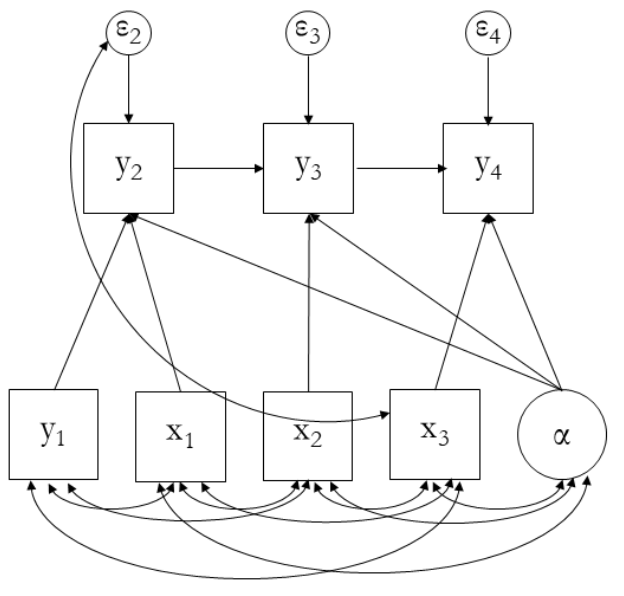
\includegraphics[width = 0.65\textwidth, height = 8cm]{Figures/Methodology/Sequential Ignorability.png}
    \label{fig:SeqIgnor}
    \caption*{\footnotesize{Note. All variables with dotted lines are assumed to be endogenous factors, capable of moderating the ODA effectiveness on health outcome.\\ Allison eta= al 2018.}}
\end{figure}

Therefore, to address both feedback and carryover effects, the autoregressive parameter (effect of $y_{it-1}$ on $y_{it}$) is controlled and  $x_{it}$ is treated predetermined or sequentially exogenous variable, as shown DPM Equation \ref{eq3}:

%given the intricate relationship between the variables of interest, this thesis employs a dynamic panel model alongside the fixed effect model. In the framework of a dynamic panel model (Figure \ref{fig:SeqIgnor}), Equation 4 can be expressed as:


\begin{equation}
    y_{it} = \delta y_{it-1} + \beta_{1} x_{it} + \theta z_{it} + \mu_i + \lambda_t + \epsilon_{it}
    \label{eq3}
\end{equation}

Here, $x_{it}$ being predetermined or sequentially exogenous implies that  $E[\epsilon_{it}|x_{it}, \mu_i] = 0$, for all $s \geq t$ \parencite{allison2017maximum}. In other words, $x_{it}$ is allowed to correlate with past error, but exogenous of current or future error \parencite{seddig2020maximum}. Notably, controlling for the autoregressive parameter (past outcome) as a predictor introduces additional endogeneity since both contemporaneous ($y_{it}$) and past ($y_{it-1}$) health outcomes are functions of and correlated with country characteristics, $\mu_i$ \parencite{shafa_assessment_2023, yogo_health_2015, nwude_official_2020}.

While scholars do not unanimously agree on a singular approach to address the endogeneity problem in dynamic panel analysis, econometricians commonly and popularly have employed instrumental variables (IV), particularly based on the first difference and system General Method of Moments (GMM) of Arellano-Bond (AB) approach for decades \parencite[see][]{arellano1991some, alonso1999symmetrically, allison2017maximum}. While the first difference AB method eliminates unit FE parameter, $\mu_i$ \parencite{arellano1991some}, system AB GMM uses both level and difference equations. However, recent studies based on simulations, have revealed significant weaknesses of IV-based and moment conditioning models. According to them, the major setbacks of GMM: are small-sample bias, particularly when panel wave, $t$, is small, and when autoregressive parameter, $\delta$, is close to 1.0 and sensitivity of the model to instruments \parencite{allison2017maximum, seddig2020maximum, becker2023many}.  Against this backdrop, the thesis adopts the Fixed Effect Cross-Lag Model (FE-CLM) of \textcite{allison2017maximum}, an approach based on maximum likelihood estimation of structural equation model (ML-SEM) specificy in Equation \ref{eq4}:
\begin{equation}
\begin{split}
    y_{it} = \delta y_{it-1} + \beta x_{it-1} + \theta z_{it} + \mu_i + \lambda_t + \epsilon_{it}\\
 x_{it} = \delta y_{it-1} + \beta x_{it-1} + \theta m_{it} + \rho_i + \tau_t + \epsilon_{it}
 \end{split}
    \label{eq4}
\end{equation}
The approach includes both the autoregressive ($\delta y_{it-1}$) and cross-lag ($\beta x_{it-1}$) parameters and employs a structural equation model with maximum likelihood estimation (ML-SEM) to analyze the causal predominance of lagged effect of $x$ and $y$ \parencite{seddig2020maximum}. The plausibility of this approach is that, first, it assumes multivariates normality of all endogenous variable $x_{it}$ and $y_{it}$, and even if the assumption is violated, ML-SEM produces a consistent and asymptotic estimate \parencite{allison2017maximum}. Furthermore, ML-SEM relaxes AB assumptions of temporal dynamics of the error variances at each time period. Finally, ML-SEM requires no specific instrumental variables  \parencite{allison2017maximum, becker2023many, moral2019dynamic}. 



%$t-j$, $j = 1, 2, 3...J$, refers to past or lagged values of the respective variables, $\delta$ for the vector of lagged health outcomes, and $\beta_{1}$ for lagged treatment (ODA allocation). In this model, as strict exogeneity fails ($E[\epsilon_{it}|x_{it}] \neq 0$), sequential ignorability allows us to assume that ODA is sequentially exogenous ($E[\epsilon_{it}|x_{it-j}] = 0$) \parencite[see][]{blackwell2018make, becker2023many, allison2017maximum}. 


%and the Fixed Effect Cross-Lag Model (FE-CLM) \parencite[see][]{allison2017maximum, becker2023many, moral2019dynamic}. Although the FE-CLM is considered to produce a superior and more consistent estimate, especially concerning the small sample bias of the AB method, it encounters significant convergence problems and computational difficulties \parencite{nino2022aid}. Consequently, this thesis adopts the system GMM proposed by \textcite{blundell1996econometric}. The AB GMM method utilizes an instrumental variable to address the endogeneity of the autoregressive parameter and country FE \parencite{nwude_official_2020, yogo_health_2015}. The system GMM represents an extension of the first difference GMM, offering higher asymptotic efficiency \parencite{nwude_official_2020}.


%$t-j$, $j = 1, 2, 3...J$, refers to past or lagged values of the respective variables, $\delta$ for the vector of lagged health outcomes, and $\beta_{1}$ for lagged treatment (ODA allocation). In this model, as strict exogeneity fails ($E[\epsilon_{it}|x_{it}] \neq 0$), sequential ignorability allows us to assume that ODA is sequentially exogenous ($E[\epsilon_{it}|x_{it-j}] = 0$) \parencite[see][]{blackwell2018make, becker2023many, allison2017maximum}.



\subsection*{4.3  Model Specifications and Hypotheses}
\addcontentsline{toc}{subsection}{4.3 Model Specifications and Hypotheses}
\subsubsection*{\quad 4.3.1 Hypothesis One}
The overarching objective of the thesis is to assess the impact of ODA on health outcomes. Given the multiple dimensions employed to measure health outcomes, the hypothesis for the research question is:

\begin{itemize}
    \item[i.] \(H_0\): \textit{ODA does not significantly affect at least one dimension of health outcomes in developing countries.}
\end{itemize}
To test this hypothesis, the thesis employs two approaches: first, the fixed effect cross-lag panel method with ML-SEM Equation in \ref{eq4} is re-specified in Equation \ref{eq5} below, with total ODA:   

%a basic sequential exogenous model with a two-way Fixed effect\footnote{Note: The first line of Equation \ref{eq5} is not a full Dynamic Panel Model (DPM) but a basic dynamic model to ensure that ODA is sequentially exogenous in predicting health outcomes without allowing the disturbance term \(\epsilon_{it}\) to correlate with ODA. The major element of a dynamic model is the autoregressive parameter \(\delta\) in Equation 5.}  and a dynamic model in eq. \ref{eq5}:

\begin{equation}
    HO_{it} = \delta HO_{it-1} + \beta_{1} ODA_{it-1} + \theta z_{it} + \mu_i + \epsilon_{it}
    \label{eq5}
\end{equation}

As robustness checks, a simple fixed effect is employed (without the autoregressive parameter, $\delta$) with social infrastructure ODA:
\begin{equation}
    HO_{it} = \beta_{1} ODA_{it-1} + \theta z_{it} + \mu_i + \lambda_t + \epsilon_{it}
    \label{eq6}
\end{equation}
%HO_{it} &= \beta_{1} ODA_{it-j} + \theta z_{it} + \mu_i + \lambda_t + \epsilon_{it} \\        

\subsubsection*{\quad 4.3.2 Hypothesis Two}

In furtherance of the main research question above, the thesis aims to assess whether the impact of ODA varies across regions, particularly SSA and non-SSA regions. 
\begin{itemize}
    \item[ii.] \(H_0\): \textit{The impact of ODA on health outcomes is not significantly different between SSA and non-SSA regions on at least one health dimension.}
\end{itemize}
The FE-CLMP, specified in Equation \ref{eq5}, is employed to test the hypothesis II, while controlling for interactions of respective regional dummy variable and total ODA, as shown in Equation 
\begin{equation}
    HO_{it} = \delta HO_{it-1} + \beta_{1} ODA_{it-1} + \beta_2 (SSA\times ODA_{it-1})  + \theta z_{it} + \mu_i + \lambda_t + \epsilon_{it}
    \label{eq7}
\end{equation}

%+ \beta_3 (Europe\times ODA_{it-1}) + \beta_4 (MENA\times ODA_{it-1}) + \beta_5 (LCA\times ODA_{it-1}) + \beta_6 (SCA\times ODA_{it-1})
%approach to capture the regional heterogeneity of SSA and non-SSA regions, with SSA countries taking value of 1, and non-SSA taking 0. The region dummy is then controlled and interacted with ODA, as shown in eq \ref{}


Here, $\beta_1$ (non-SSA), a vector of coefficients for non-SSA regions dummy interactions with ODA and $\beta_2$, a scalar coefficient for SSA region are the parameters of interest, representing the effect of ODA in SSA and non-SSA regions. A similar approach is replicated in the ordinary fixed effect model for robustness, albeit with social infrastructure ODA and without autoregressive parameter $\delta$. 

%This hypothesis will be tested by controlling for regions. The thesis classifies all developing countries in our analysis into six regions: MENA, SSA, Europe, EAP, LAC, SCA. 


\subsubsection*{\quad  4.3.3  Hypothesis Three:}
The thesis's third and final objective is to understand the mediating role of social protection in the impact of ODA on the health dimension. Thus, the hypothesis is that:

\begin{itemize}
    \item[iii.] \(H_0\): \textit{The indirect role of Social protection in the impact of ODA on health outcome is not statistically significant for at least one health dimension.}
\end{itemize}

While \textcite{yogo_health_2015} employed female education and health spending per capita, this thesis employs social protection as the potential mechanism. To model this relationship, the mediation causal approach with fixed effect is employed, discussed in \textcite{hayes2009beyond, hicks2011causal, becker2023many}. The path analysis is shown in the Directed Acyclic Graph (DAG) in Figure \ref{DAG-mediation} below:  
\begin{figure}[!ht]
\centering
\caption{Figure 4: Mediation Path analysis}
\resizebox{0.5\textwidth}{!}{%
\begin{circuitikz}
\tikzstyle{every node}=[font=\normalsize] % Adjust font size here

\draw (7.5,17) ellipse (1cm and 0.5cm) node {\normalsize ODA};
\draw (11.5,17) ellipse (1cm and 0.5cm) node {\normalsize HO};
\draw [->] (8.5,17) -- (10.5,17);
\node at (9.5,17.25) {c'};

\draw (9.5,19.5) ellipse (0.75cm and 0.5cm) node {\normalsize SP};
\draw [->] (7.75,17.5) -- (9.25,19);
\draw [->] (9.75,19) -- (11,17.5);
\node at (8.05,18.55) {a};
\node at (11.05,18.25) {b};

\draw [, dashed] (11.75,21.25) circle (0.5cm) node {\Large $\epsilon_1$};
\draw [, dashed] (14.5,18.25) circle (0.5cm) node {\Large $\epsilon_2$};
\draw [-Stealth, dashed] (11.25,20.75) -- (10.25,19.75);
\draw [-Stealth, dashed] (14,18) -- (12.5,17.25);
\end{circuitikz}
}%
\label{DAG-mediation}
\end{figure}

Path $c'$ represents the direct impact of ODA on health, path $a$ for ODA impact on social protection and path $b$ for the effect of social protection on health. The causal order is represented as follows: \(ODA_{it-4} \rightarrow SP_{it-3} \rightarrow HO_{it}\)\footnote{Note that, the causal order is a mere assumption, which may not necessarily be true \parencite[see][]{yogo_health_2015}.}. The total effect = \(c' + a\times b \), here, the main parameter of interest (social protection as mechanism) is the joint significance of $a \times b$. If they are both significant and the effect of ODA on health is reduced after controlling for Social protection, then social protection is a significant channel of ODA effect on health \parencite[see][]{becker2023many, yogo_health_2015}. 


\subsection*{4.4 Variable Selection, and Data Sources}
\addcontentsline{toc}{subsection}{4.4 Data, Variable Selection and Data Sources}
This thesis utilizes relevant secondary data for 144 developing countries, in Appendix C Table \ref{tab:country_info}, all of which are classified as ODA eligible by \textcite{oecd_Data_2023}. The dataset spans  22 years, between 2000 to 2021, a period chosen to align with the inception of the Sustainable Development Goals (SDG) in 2000. It's noteworthy that ODA data dates back further than SDG and the descriptive analysis of ODA in Chapter Two incorporated earlier data, starting from 1990. All study variables fall in three categories: the dependent variable (health outcomes); the main independent variable (ODA); and the control variables, also known as covariates. 

\subsubsection*{\quad 4.4.1 Dependent Variable: Health outcomes}
As outlined earlier, health is a complex and multidimensional concept. The literature review section unveils narrow indicators used to proxy health outcomes in prior studies (See Literature review section for details). For example, \textcite{nwude_official_2020} focused on life expectancy and under-5 mortality, while \textcite{odokonyero_impact_2018, bavinger_relationship_2017} used the burden of diseases, \textcite{doucouliagos_health_2021} utilized infant mortality, and \textcite{kavakli_us_2022} used family planning as a proxy for health outcomes. However, these indicators lack depth to adequately capture the diverse and nuanced nature of health across different regions. Furthermore, such narrow indicators may obscure the true impact of ODA.

Consequently, this thesis adopts a more holistic approach to measuring health. Specifically, Sustainable Development Goal (SDG) 3, on health and well-being, and SDG 2.3 on malnutrition are employed as proxies for health. These indicators provide a robust framework encompassing various health dimensions, facilitating an in-depth exploration of the impact of ODA on diverse aspects of health in developing countries. After the initial variable selection and correlation analysis, 26 health and malnutrition indicators, listed in Appendix A.2 Table \ref{Tab::health indicators}, were retained and subsequently used to construct six composite health dimensions. Appendix B Figure \ref{fig:combined_scat_plot}, illustrates the distribution of countries across respective health dimensions. See the discussion on respective health dimensions in Chapter Two and the procedure for the composite health dimensions in Appendix B.1.

The health dimensions constructed-reproductive risk and fatalities (RFTP), malnutrition, burden of infection and diseases (BID), health system capacity and responsiveness (HSCR), environmental death, and burden of mental problem (BMP)—each contribute to a comprehensive understanding of health outcomes. This approach elucidates the nuanced nature of health across world regions and the dynamic of ODA effectiveness on the diverse health dimensions. All health indicators were primarily sourced from the United Nations Sustainable Development Statistics (UNSDG) \parencite{unsdg_sustainable_2023}, the global database for data on SDG goals. To address the high levels of missing data for certain indicators in the UNSDG, the World Bank's World Development Indicators (WDI) database \parencite{wdi_world_2023} was utilized to supplement the dataset.

\subsubsection*{\quad 4.4.2 Independent Variables} 
\paragraph{\quad \quad \textit{4.4.2.1 Official Development Assistant (ODA)}}
\subparagraph{}
The main independent variable in this study is ODA, otherwise known as foreign aid, which is the financial and technical support provided by affluent countries for developmental purposes in developing nations. See Chapter Two for a discussion on ODA and its classification system in Appendix A.1 Figures \ref{fig:General ODA classification} and \ref{fig:Sector ODA classification}. While there is no consensus on the specific type of ODA to use when assessing its impact on health, many previous studies \parencite[e.g.,][]{nwude_official_2020, odokonyero_impact_2018} employed health ODA. Others, including \textcite{yan_mortality_2015, kavanagh_governance_2019, ali_foreign_2020, yogo_health_2015}, utilized the Global Health Fund, and \textcite{cassola_evaluating_2022} focused on research ODA. Additionally, \textcite{bavinger_relationship_2017} considered child health ODA, \textcite{marty_taking_2017} explored infrastructure and parasitic ODA, and \textcite{staicu2017study, akinola_foreign_2022} investigated total ODA. 

%Coefficients of ODA are expected to be negative for all health dimensions, but positive for health system capacity and responsiveness (HSCR)

As illustrated in Appendix A.1 Figure \ref{fig:Sector ODA classification}, health ODA constitutes only a small subsector of social infrastructure ODA. Additionally, other subsectors within social infrastructure ODA, apart from health, have elements of health. Therefore, this thesis, following preceding studies \textcite{williamson_foreign_2008, toseef_how_2019, doucouliagos_health_2021}, employed both total net and social infrastructure ODA. Net ODA is chosen over total disbursement to account for repayment over time. All ODA data were sourced from the OECD database \parencite{oecd_Data_2023}.

\paragraph{\quad \quad \textit{4.4.2.2 Social Protection}}
\subparagraph{}
In this study, social protection is hypothesized as a mediating channel through which ODA may impact health. While mediation analysis is relatively scarce in previous studies assessing the impact of ODA on health, studies, including \textcite[]{mahembe_foreign_2019, forte_impact_2023}, on ODA and social protection have rarely utilized explicit social protection indicators. Instead, many previous studies employed poverty and income per capita as proxies for social welfare. This choice is often attributed to the limited availability of panel data specifically focused on social protection, as highlighted by \textcite{nino-zarazua_aids_2023}. Similar to \textcite{nino-zarazua_aids_2023}, the thesis utilizes the coverage of all social protection as a proxy for social protection development in developing countries. The variable is measured as \% of the total population with access to any form of social protection and the data is sourced from the World Bank Aspire database \parencite{wdi_world_2023}. The coefficient of both ODA and social protection are expected to be negative for all health dimensions, except HSCR.  
 
\subsubsection*{\quad 4.4.3 Control Variables}
%\addcontentsline{toc}{subsubsection}{ 4.4.3 Control Variables}
The third classification of variables is covariates, also known as control variables. In this study, covariates are confounding factors affecting both ODA and health outcomes. They mitigate omitted variable bias (OVB) in the model and ensure baseline equivalence among study units. All control variables, except the Climate Risk Index (CRI) are sourced from the World Development Indicators \parencite{wdi_world_2023}. The following are the controlled variables considered in this study:

\begin{enumerate}[i]
    \item \textbf{GDP per Capita:} GDP per capita is fundamental to accounting for the initial level of economic development in a country. An increase in countries' GDP Per capita enhances their health outcome and reduces their likelihood of receiving ODA \parencite{oecd_ODA_Report_2023}. This variable, used in numerous reviewed studies \parencite[e.g.,][]{williamson_foreign_2008, nwude_impact_2023, toseef_how_2019}, is measured in 2017 constant price US dollars \textcite{wdi_world_2023}. The variable is logged in the model to address high skewness.
   % \item \textbf{Government Health Spending:} Domestic government health expenditure signifies the level of a country's commitment to its healthcare system. This spending not only influences the strength of the healthcare system but also impacts health outcomes, as used in previous studies \parencite{yan_mortality_2015, chung_economic_2022, mohamed_foreign_2017, akinola_foreign_2022}. The variable is measured as a percentage of total health spending in 2017 constant price \textcite{wdi_world_2023} and logged in the model.  
    \item \textbf{Domestic government health finance capacity:} The thesis employs both domestic government health spending per capita and stock of external debt, as a proxy for countries' public finance. While government health spending per capita signifies the level of a country's commitment to its healthcare system, \parencite[see][]{yan_mortality_2015, mohamed_foreign_2017, akinola_foreign_2022}, the external debt stock exerts downward pressure government's capacity to invest in the health system \parencite{kumar2010public, ogunjimi2019impact}. Surprisingly, prior studies did not control for government debt, despite its significant influence on public health finance in developing countries \parencite{kumar2010public}. Government spending per capita is measured in 2017 constant price, external debt is measured as per GNI \parencite{wdi_world_2023}. Both variables are logged to mitigate skewness.   
    
   % \item \textbf{Log(External Debt Stock):} A crucial factor influencing the public finance and investment capacity of many developing countries is public debt. In an IMF-published study, \textcite{kumar2010public} revealed a negative relationship trend between the external public debt-to-GDP ratio and economic growth. Specifically, a 10 percentage point rise in the initial debt-to-GDP ratio led to a 0.2 percentage point annual reduction in real per capita GDP growth \parencite{kumar2010public}. A more detailed negative impact of external debt is uncovered in a study by \textcite{ogunjimi2019impact} in Nigeria. Surprisingly, prior studies did not control for government debt, despite its significant influence on public health finance in developing countries. The variable is measured as a percentage of the country's GNI and sourced from the World Development Indicators \parencite{wdi_world_2023}. The thesis applies a logarithmic transformation to the variable to mitigate the impact of skewness caused by extreme debt-ridden countries.
    
    \item \textbf{Demographic factors:} Country size, proxy by population, and population density are crucial to countries' health outcomes. Countries with higher populations often strain healthcare systems. Population density may support healthcare infrastructure development, enhancing accessibility to medical facilities, but may also contribute to the spread of infectious diseases and inadequate sanitation, negatively affecting health. While  \textcite[e.g.,][]{staicu2017study, chung_economic_2022, yogo_health_2015, doucouliagos_health_2021} controlled for population as a proxy of country size, \textcite{doucouliagos_health_2021} employed both population and population density. Both variables are logged in the models.
 %   
  %  Higher populations often strain healthcare systems and correlate with increased health problems. This variable is measured in absolute values and sourced from the World Development Indicators \parencite{wdi_world_2023}. Despite its high correlation with other demographic variables, the population is retained due to its significance. The logarithmic transformation is applied to address skewness. Noteworthy, this variable exhibits a positive effect on all health dimensions, with a specific positive impact on HSCR.
   % \item \textbf{Log(Population Density):} Another vital social demographic factor influencing health is population density, in accordance with previous studies \parencite{toseef_how_2019, doucouliagos_health_2021}. The thesis controls for population density, measured as people per square kilometer of land area, with data sourced from the World Development Indicators \parencite{wdi_world_2023}. To address skewness, a log transformation is applied.
    %Higher population density can have a dual impact: it may support healthcare infrastructure development, enhancing accessibility to medical facilities, but it can also contribute to the spread of infectious diseases and inadequate sanitation, negatively affecting health. Consequently, the thesis anticipates a negative association of population density with all health dimensions, while expecting a positive effect on health system capacity and responsiveness.
    
    \item \textbf{Infrastructure development:} The level of infrastructure development plays a crucial role in the overall health and well-being of citizens. While \textcite{doucouliagos_health_2021, yogo_health_2015} controlled for sanitation and water access, \textcite{odokonyero_impact_2018, yan_mortality_2015, williamson_foreign_2008} employed urbanization to measure infrastructure development. As utilized by \textcite{toseef_how_2019} and due to the high correlation of electricity access with various development indicators, including education, sanitation and water access, HDI etc, the thesis employs electricity access as a proxy of the infrastructure development level of countries.  Electricity access is measured as the percentage of the population with access to electricity \textcite{wdi_world_2023}. 
    
    \item \textbf{Alternative foreign inflow:} Foreign Direct Investment (FDI) and remittance are crucial alternative foreign inflows in developing countries \parencite{scott_lessons_2020}, capable of bolstering investment capital and strengthening health systems and outcomes. The nature of impact of all foreign inflows depends on the recipients of those flows: while remittance flows to households \parencite[see][]{obi2020does, gamlen2014new, de2009remittances}, FDI encourages flow technology \parencite{chung_economic_2022} and ODA flow more to the government. Regardless, all foreign inflows, regardless of their nature, have an enormous impact on health outcomes and the well-being of developing countries, thus making FDI and remittances crucial in the thesis models.   
    
    %While \textcite{yogo_health_2015} controlled for remittance per capita, remittances typically don't directly contribute to government funds, limiting their impact on public health investment and overall national development \parencite[see][]{obi2020does, gamlen2014new, de2009remittances}. In alignment with \textcite{chung_economic_2022}, this thesis opts for FDI as an alternative foreign financial flow. The variable is measured as net inflows as a percentage of GDP, with data sourced from the World Development Indicators \parencite{wdi_world_2023}.
    
    \item \textbf{Climate Risk Index Score:} The Climate Risk Index (CRI) Score ranks countries and regions based on their vulnerability to the impacts of climate change, particularly extreme weather events like storms, heatwaves, and floods \parencite{eckstein2021global}. The escalating impact of climate change on global health cannot be overstated. While \textcite{nwude_official_2020} controlled for CO$_2$ emissions, the thesis contends that the impact of climate change on the health of developing countries' populations is not necessarily proportional to their emissions. Hence, the thesis opts for the CRI Score, which reflects the vulnerability and exposure of developing countries to various climate impacts, likely affecting population health. The CRI Score, compiled by German Watch, ranges from 2 to 166 and is sourced from the most recent version in 2021 \parencite{eckstein2021global}. 
    
    %\item \textbf{Log(Trade per GNI):} Trade is a fundamental factor influencing the economic development, health, and overall well-being of a country. Nations with higher trade tend to exhibit positive economic and health outcomes \parencite[see][]{makki2004impact, pavcnik2017impact}. Previous studies incorporated trade in various forms, such as export value in \textcite{chung_economic_2022} and net trade values in \textcite{forte_impact_2023, shafiullah_foreign_2011}, as a proxy for countries' trade openness. In a similar vein, this thesis controls for countries' level of trade, measured as a percentage of GDP. The variable undergoes a log transformation, and raw data is sourced from the World Development Indicators \parencite{wdi_world_2023}. Trade is anticipated to have a negative effect on all health dimensions but a positive impact on health system capacity and responsiveness.
    
    \item \textbf{Quality of governance:} The impact of institutional/governance quality continues to be debated \parencite[e.g.][]{doucouliagos_health_2021, williamson_foreign_2008}. Previous studies have employed various governance proxies, such as control of corruption, Fraser freedom index, civil conflict, political regimes, and democracy index sourced from the World Development Indicators \parencite{shafiullah_foreign_2011, muhammad_health_2021, toseef_how_2019, williamson_foreign_2008, kavakli_us_2022, yogo_health_2015}. In this thesis, governance quality is proxied by the general Governance Index, which allows inter-country comparisons across six crucial governance dimensions: voice and accountability, political stability and absence of violence, government effectiveness, regulatory quality, rule of law, and control of corruption \parencite[see][for detailed description of the index]{handoyo2023worldwide, wdi_world_2023}.
\end{enumerate}









     
       






 
 



\subsection*{4.5 Data Analysis Tools}
\addcontentsline{toc}{subsection}{4.5 Data Analysis Tools}
The thesis employs R-programming for data analysis. Key packages utilized include SDG and WDI,  used for loading data from the World Bank and UN statistics. Tidyverse was used for all data transformation and plots. MisForest was employed for imputing missing values; Plm and DPM for econometric analysis and hypothesis testing; LmTest for robust standard error estimation due to heteroscedasticity. Also, Groundhog was used to keep packages updated to ensure the reproducibility of findings. All code scripts for the data analysis are submitted alongside the thesis. 






%\subsubsection*{General Panel Tests for Model Specification}

%Multicollinearity test, Poolability/Panel Test, Homoscedasticity test, Serial Correlation test, and stationarity test.

%(individual time varying characteristics varies across units and time dimensions which is the error term in FE)
